\section{Data Set}\label{dataset}

We use Telecom Churn Dataset in our research. This is a data of a Telecom company Orange of their USA customers and it is publicly available via Kaggle.com. 
The Orange Telecom's Churn Dataset, which consists of cleaned customer activity data (features), along with a churn label specifying whether a customer has canceled the subscription or not.

Two datasets are made available: the “churn-bigml-80” and “churn-bigml-20”. The two sets are from the same batch, but have been split by an 80/20 ratio. Furthermore, in our research, we split the “churn-bigml-80” data set by another 75/25 ratio for training and validation purposes. Hence we have 60% for training, 20% for validation and 20% of data for testing.

The "churn-bigml-80" data set contains 2666 observations, each representing a customer, and 20 variables (features). The "churn-bigml-20" data set contains 667 observations (customers) and 20 variables (features). The "Churn" column is the target variable that we would like to predict. It has two levels: “True” for confirmed churn (customer has left the company) and “False” for retained customer (stayed with company). \newline
\newline
The data sets have the following attributes or features: \newline \newline
\textbf {State:} factor	\\
\textbf {Account length:} integer \\
\textbf {Area code:} integer \\
\textbf {International plan:} factor \\
\textbf {Voicemail plan:} factor \\
\textbf {Number vmail messages:} integer\\
\textbf {Total day minutes:} double \\
\textbf {Total day calls:} integer \\   
\textbf {Total day charge:} double \\
\textbf {Total eve minutes:} double \\
\textbf {Total eve calls:} integer \\
\textbf {Total eve charge:} double \\
\textbf {Total night minutes:} double \\ 
\textbf {Total night calls:} integer \\
\textbf {Total night charge:} double \\
\textbf {Total intl minutes:} double \\ 
\textbf {Total intl calls:} integer \\
\textbf {Total intl charge:} double \\
\textbf {Customer service calls:} integer \\
\textbf {Churn:} factor \\

\newpage
As part of our data preparation process, we convert our variable names to all lower case names (for readability) and variable types: 

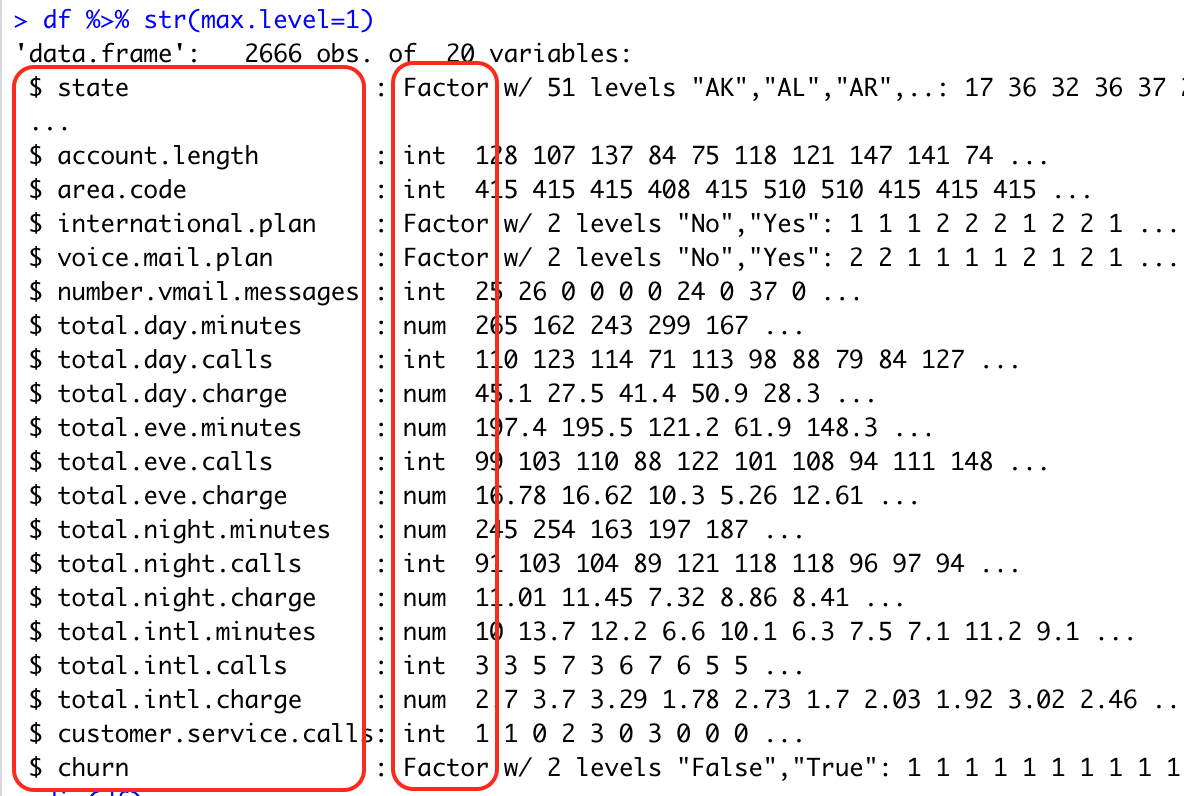
\includegraphics[width=\linewidth]{Picture_1.png}


We also need to make sure that the proportion of entries for each class in the “churn” variable is the same for training/validation data frame and for testing one. 

\begin{verbatim}
There are 2278 “False” churns (customers who didn't leave/stayed with the company) and 388 “True” churns (where customers actually left the company) in the train data frame. This is about 85% and 15% respectively. Test data frame contains 572 (86%) of “False” churns and 95 (14%) of “True” churns. So the representation of entries for each class is proportional in each data frame.
\end{verbatim}
